\documentclass[]{article}
\usepackage{caption,subcaption,graphicx,float,url,amsmath,amssymb,amsthm,tocloft,cancel,thmtools,gensymb,braket}
\usepackage[toc,nonumberlist]{glossaries}
\usepackage{glossaries-extra}
\newcommand\numberthis{\addtocounter{equation}{1}\tag{\theequation}}

\newtheorem{thm}{Theorem}
\newtheorem{defn}[thm]{Definition}
\newtheorem{cor}[thm]{Corollary}
\newtheorem{lemma}[thm]{Lemma}
\graphicspath{{figs/}}
\widowpenalty10000
\clubpenalty10000
\setcounter{tocdepth}{2}

%opening
\title{Theoretical Minimum\\Particle Physics 1\\Basic Concepts}
\author{Simon Crase(compiler)}

\begin{document}

\maketitle

\begin{abstract}
These are my notes for \emph{New Revolutions in Particle Physics 1} lectures from Leonard Susskind's Theoretical Minimum series.
\end{abstract}

\tableofcontents
\listoffigures
\listoftables
\listoftheorems

\section{Particles and Light}

This lecture contains  facts from other courses, which will be used on later lectures.

Particle physics is about the question: is matter discrete? If so we will call the smallest things "particles". If matter forms a continuum, we have fields.

Which is correct? Both and neither.

First evidence for atoms came from chemistry. John Dalton looked at mass mole: each substance was an integer multiple of mass of a mole of hydrogen; it suggested that there are building blocks. We now know that mass of molecule is mass of protons, electrons (very small), and neutrons, which have nearly the same mass as protons. 
 
Figure \ref{fig:em:wave} illustrates an electromagnetic wave. We need the concepts of wavelength, $\lambda$, and period, $T$.

We have
\begin{align*}
\frac{\lambda}{T}=&c\\
f=&\frac{1}{T} \text{, so}\\
\lambda f =& c\text{. Physicists tend to measure frequency in radians per second:}\\
\omega =& 2 \pi f \text{, so} \\
\omega =& \frac{2 \pi c}{\lambda} \numberthis \label{eq:omega:lambda}
\end{align*}

\begin{figure}[H]
	\caption{An electromagnetic wave}\label{fig:em:wave}  
	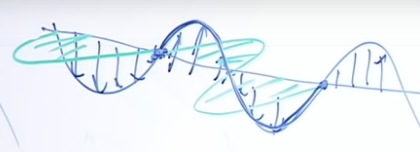
\includegraphics[width=0.9\textwidth]{Wavelength}
\end{figure}

Wave/particle duality.

A photon has energy:
\begin{align*}
E=&\hslash \omega \text{. Energy of single photon.} \numberthis\label{eq:E_omega}\\
E_{ray}=&n \hslash \omega \text{. Energy of ray.}
\end{align*}
 

In modern usage, mass is what used to be called rest mass. $E = m c^2$ only for stationary object.

In particle physics we choose units to set $c=1$ and $\hslash=1$. In this lecture $c$ and $\hslash$ will appear explicitly only when Prof. Susskind wants to show the magnitude of some quantity.

Energy depends on the motion of the object as seen by the observer: it isn't a universal thing that everyone will agree on.

Light has energy and momentum (not mass): 

\begin{align*}
\left|P\right|=&\frac{E}{c} \\
=&\frac{\hslash \omega}{c} \text{, from (\ref{eq:E_omega})}\\
=& \frac{2 \pi \hslash}{\lambda} \text{, from (\ref{eq:omega:lambda}). c.f. Harmonic Oscillator.}\numberthis\label{eq:P:lambda}
\end{align*}

This is why we need larger and larger instruments to observe smaller particles!
To see really small things, we need particles with high energy and momentum.


\section{Quantum field theory}

\subsection{Mathematical Preliminaries}

Consider a classical wave $A \sin(kx)$. Energy is $A^2$, but it is also proportional to number of photons, $n$: $E \propto n \hslash \omega$, $A \propto \sqrt(n)$.

Generally, equations containing $c$ apply for photons only. For non-relativistic particles:
\begin{align*}
E=&\frac{p^2}{2m}\\
f =& \frac{h}{2 m \lambda^2} \text{. c.f. Schr\"odinger equation!}
\end{align*}

\begin{itemize}
	\item Phase Velocity: velocity of wave packet;
	\item Group velocity: velocity of troughs and peaks--identified with particle velocity.
\end{itemize}

For light waves, phase and group velocities the same, but this isn't true for most particles. Phase velocity can exceed $c$, but can't transmit information.

Space is infinite. But physics is the art of getting problems into a shape that computers can solve, so we need to remove infinities.

Let's look at 1 dimensional waves. We can restrict to fixed length $L$: reflecting boundary condition at ends. But this violates conservation of momentum. Instead use a topological "circle" circumference $L$--periodic boundary conditions. As a consequence momentum is quantized: 

\begin{align*}
\lambda =& \frac{L}{N}\\
P =& \frac{h}{\lambda}\\
=& \frac{h N}{L}
\end{align*}

Now make into a real circle, radius $R$, and redefine $L$ to be \emph{angular momentum}.

\begin{align*}
P =& \frac{h N}{2 \pi R}\\
L =& N \frac{h}{2 \pi}\\
=& N \hslash \text{ independent of $R$.}
\end{align*}

\subsection{Quantum field theory}

Start with harmonic oscillator: a wave is a collection of harmonic oscillators. Energy is quantized: 0, $\hslash \omega$, $2\hslash \omega$...

Introduce operators:

\begin{align*}
a^+ \ket{n} =& \sqrt{n+1} \ket{n+1} \text{, creation operator} \numberthis \label{eq:creation}\\
a^- \ket{n} =& \sqrt{n} \ket{n-1} \text{, annihilation operator} \numberthis \label{eq:annihilation} \\
a^+ a^- \ket{n} =& n \ket{n} \text{, or}\\
a^+ a^-  =& n \text{, similarly}\\
a^- a^+  =& n+1\\
[a^-, a^+] =& 1
\end{align*}

Return to world on a circle--$\omega_N$--equivalent to oscillator. State is $\ket{n_1,n_2, n_3,...}$--occupation numbers. 
\begin{defn}[quantum field]
	A quantum field is a collection of harmonic oscillators, togther with annihilation operators and creation operators.
\end{defn}

\section{Quantum fields and particles}



\begin{align*}
\text{Wave} =& e^{i k x} \text{, $k$ is wave number}\\
P=&\hslash k\\
n(k) =& \text{ occupation number.}
\end{align*}

We represent the state of a 1D circular system by occupation numbers, $\ket{...n(-1), n(0), n(1), n(2)...}$, and introduce operators $a^+(k)$, $a^-(k)$. 
\begin{align*}
a^+(1)\ket{...n(-1), n(0), n(1), n(2)...}=& \sqrt{n(1)+1}\ket{...n(-1), n(0), n(1)+1, n(2)...}
\end{align*}
$a^+(k)$, $a^-(k)$ are quantum mechanical versions of the Fourier coefficients of a field $\Psi$.

Here is a classical wave:
\begin{align*}
\Psi(x) =& \sum_k \alpha(k) e^{ikx}\\
\Psi^*(x) =& \sum_k \alpha^*(k) e^{-ikx}
\end{align*}

We quantize as shown in (\ref{eq:q:1}) and (\ref{eq:q:2}) to produce a quantum field:
\begin{align*}
\alpha(k) \rightarrow& a^-(k) \numberthis \label{eq:q:1}\\
\alpha^*(k) \rightarrow& a^+(k) \numberthis \label{eq:q:2}\\
\Psi(x) =& \sum_k a^-(k) e^{ikx} \numberthis \label{eq:Psi}\\
\Psi^\dagger(x) =& \sum_k a^+(k) e^{-ikx} \numberthis \label{eq:Psi:dagger}
\end{align*}

We need to justify (\ref{eq:q:1}) and (\ref{eq:q:2}) in some appropriate limit.

How can we describe scattering? Imagine scattering so a particle with momentum $k_7$ becomes a particle with momentum $k_9$: $a^+(k_9)a^-(k_7)\ket{0,0,..1,0,0}$.

What if laws of physics allows number of particles to change? $a^+(k_{16})a^+(k_9)a^-(k_7)\ket{0,0,..1,0,0}$. We can't do this in regular quantum mechanics.

What does $\Psi^\dagger$ do? Start with the vacuum $\ket{0}$.

\begin{align*}
\Psi^\dagger(x)\ket{0} =& \sum_k a^+(k) e^{-ikx} \ket{0} \text{ from (\ref{eq:Psi:dagger})}\\
=& \sum_k e^{-ikx} \underbrace{a^+(k) \ket{0}}_\text{One particle state with momentum $k$} \\
=& \sum_k e^{-ikx} \ket{k} \text{. Superposition gives particle at definite position.}
\end{align*}

If we make the circle larger and larger, $\sum \rightarrow \int$.

What does $\Psi$ do? It annihilates a particle at $x$.

Locality: when something happens, it happens at one spot. Figure \ref{fig:ex:locality} is an example of one particle being replaced by two.

\begin{figure}[H]
	\caption{Example of locality: $\Psi^\dagger(x)\Psi^\dagger(x)\Psi(x)\ket{...}$}\label{fig:ex:locality}
	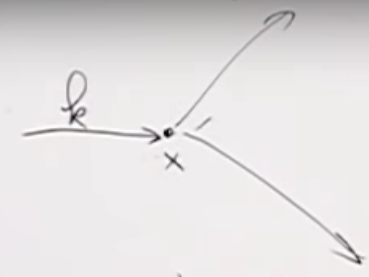
\includegraphics[width=0.8\textwidth]{split-particle}
\end{figure}

Start with state $\ket{0,...\underbrace{1}_\text{particle with momentum $k$},0,000}$.

We assume that $k_i$ denotes the index of the only momentum with a non-zero index.
\begin{align*}
\Psi^\dagger(x)\Psi^\dagger(x)\Psi(x)\ket{0,...1,0,000}=&\sum_m a^+(m) e^{-imx} \sum_l a^+(l) e^{-ilx} \sum_k a^-(k) e^{ikx} \ket{...}\\
=&\sum_m a^+(m) e^{-imx} \sum_l a^+(l) e^{-ilx} a^-(k_i) e^{ik_ix} \ket{...}\\
=&\sum_m a^+(m) e^{-imx} \sum_l a^+(l) e^{-ilx}  e^{ik_ix} \ket{0}\\
=&\sum_{l,m}  e^{-imx}  e^{-ilx}  e^{ik_ix} \underbrace{\ket{001001...}}_\text{$l$ and $m$ are indices of $1s$.}\\
\triangleq &\sum_{l,m}   e^{i(i_k-l-m)x} \ket{l,m}
\end{align*}

This isn't true if $l=m$! We have two application of $a^+(m)$, so vacuum becomes $\sqrt{2}\ket{...2...}$. Probability of two particles coming out in same state is twice probability of them being in different states.

Ignore conservation laws!

Consider generating photon at a position where there is a pre-existing photon with momentum $l$--Figure \ref{fig:simple:decay}.
\begin{figure}[H]
	\caption{Generating photon at a position where there is a pre-existing photon with momentum $l$.}\label{fig:simple:decay}
	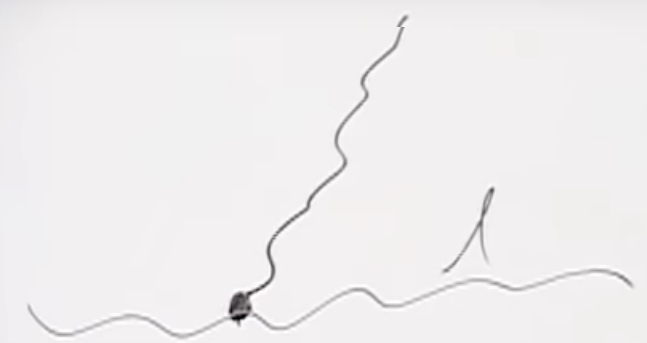
\includegraphics[width=0.8\textwidth]{decay}
\end{figure}

\begin{align*}
\Psi(x)\ket{l} =& \sum_k a^+(k) e^{-ikx} \ket{l}\\
=& \sum_{k\ne l} e^{-ikx} \ket{k,l} + \sqrt{2} e^{-ilx} \ket{l,l}
\end{align*}

Stimulated emission: higher probability of generating particles that are already there (c.f. spontaneous emission). This is true for Bosons, but not Fermions.
 
 Laws for Bosons
 \begin{align*}
 [a^+(k),a^+(l)] =& 0\\
 [a^-(k),a^-(l)] =& 0\\
 [a^-(k),a^+(l)] =& \delta_{k,j}\\
 \Psi(x) =& \sum_k a^-(k) e^{ikx} \\
 \Psi^\dagger(x) =& \sum_k a^+(k) e^{-ikx}
 \end{align*}
 
 \begin{align*}
 \frac{1}{L}\int dx \Psi^\dagger(x) \Psi(x) =& \int  \sum_k a^+(k) e^{-ikx} \sum_l a^-(l) e^{ilx}\\
 =&  \sum_k \underbrace{a^+(k) a^-(k)}_\text{Occupation number}\\
 =& N \text{, total number of particles.}\\
 \Psi^\dagger(x) \Psi(x) =& \text{ density of particles at $x$}.
 \end{align*}

\url{https://youtu.be/UgPBUJRrYz8?t=5689}


\section{More quantum field theory}

How is this related to energy and momentum conservation?

\subsection{Mathematical Preliminaries}

\subsubsection{Dirac Delta function}

\begin{align*}
\text{For } k =& \frac{2 \pi n}{L}\\
\int_{-\frac{L}{2}}^{\frac{L}{2}} e^{ikx} dx =& L \text{, if $k =0$}\\
=& 0 \text{, otherwise}\\
\rightarrow& 2 \pi \delta(k) \text{ as $k \rightarrow \inf$}
\end{align*}

We will use ket vectors for initial states, bra for final. This will help with bookkeeping.

\subsubsection{Creation and annihilation operators operating on bra vectors}

\begin{align*}
\braket{n|m} =& \delta_{n,m}\numberthis \label{eq:orthogonal} \text{. We want the following}\\
\braket{n|(a^+|m)} =& \braket{(n|a^+)|m} \text{ from (\ref{eq:creation})} \numberthis \label{eq:consistency}\\
\braket{n|(a^+|m)} =& \sqrt{m+1} \braket{n|m+1}\\
=& \sqrt{m+1} \delta_{n,m+1} \text{ from (\ref{eq:orthogonal})} \text{, so we define}\\
\bra{n} a^+ \triangleq & \sqrt{n} \bra{n-1} \text{ to satisfy (\ref{eq:consistency}), and} \numberthis \label{eq:bra:create}\\
\bra{n} a^= \triangleq & \sqrt{n+a} \bra{n-1} \numberthis \label{eq:bra:annihilate}
\end{align*}
Example: calculate an expression two different ways.
\begin{align*}
\braket{n|(a^+a^-|n)} =& \sqrt{n}\braket{n|(a^+|n-1)}\\
=& n \braket{n|n} \text{ from (\ref{eq:bra:create})}\\
=& n\\
\braket{(n|a^+a^-)|n} =& \sqrt{n} \braket{(n-1|a^-)|n}\\
=& n \braket{n|n} \text{ from (\ref{eq:bra:annihilate})}
\end{align*}

\subsection{Quantum Fields}

The only way we can study particles is to collide them; quantum field theory is the mathematical tool.

We will set $\hslash=1$, so $P=k$, and we will take $X$ and $P$ to be 3 dimensional.
\begin{align*}
\Psi^\dagger(X)(X,t) \triangleq& \sum_k a^+(k) e^{-ikX} e^{i \omega(k) t} \text{, but}\\
\omega =& E \text{ and}\\
E =& \frac{P^2}{2m} \text{, whence}\\
\omega =& \frac{k^2}{2m} \numberthis \label{eq:omega:k}\\
\Psi \triangleq& \sum_k a^-(k) e^{ikX} e^{- i \omega(k) t}
\end{align*}
We want to determine the differential equation satisfied by $\Psi^\dagger(X)$.

\begin{align*}
\dot{\Psi^\dagger(X)} =&  \sum_k i \omega(k) a^+(k) e^{-ikX} e^{i \omega(k) t}\\
\frac{\partial^2 \Psi^\dagger(X)}{\partial X^2} =& \sum_k -k^2 a^+(k) e^{-ikX} e^{i \omega(k) t} \numberthis \label{eq:omega:dot}\\
 =& - \sum_k 2m \omega a^+(k) e^{-ikX} e^{i \omega(k) t} \text{ from (\ref{eq:omega:k})}\\
 \frac{1}{2m} \frac{\partial^2 \Psi^\dagger(X)}{\partial X^2} =& - \sum_k \omega a^+(k) e^{-ikX} e^{i \omega(k) t}\\
  i \dot{\Psi^\dagger(X)} =&  \frac{1}{2m} \frac{\partial^2 \Psi^\dagger(X)}{\partial X^2} \text{ From (\ref{eq:omega:dot})--Schr\"odinger for field!}
\end{align*}

Consider particle scattering from heavy target; conserves energy, but not momentum--Figure \ref{fig:particle:heavy:target}. Assume scattering probability independent of time.

\begin{figure}[H]
	\caption{Particle being absorbed and then re-emitted}\label{fig:particle:heavy:target}
	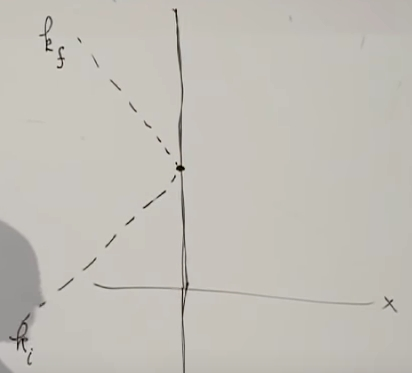
\includegraphics[width=0.8\textwidth]{particle-heavy-target}
\end{figure}

We want the probability of emitting one particle in final state (Introduce coupling constant $g$)--$\big| \bra{k_f} g \int dt \Psi^\dagger(0,t)\Psi(0,t)\ket{k_i} \big|^2$

\begin{align*}
&\bra{k_f} g \int dt \sum_l \underbrace{a^+(l) e^{i \omega_l t}}_\text{contributes iff $l==k_f$} \sum_k \underbrace{a^-(k) e^{-i \omega_k t} \ket{k_i}}_\text{contributes iff $k==k_i$}\\
=&\bra{k_f} g \int dt a^+(k_f) e^{i \omega_{k_f} t}  a^-(k_i) e^{-i \omega_{k_i} t} \ket{k_i}\\
=& g \int dt e^{i(\omega_{k_f}-\omega_{k_i})}\cancel{<0|0>}\\
=& 2 \pi g \delta(\omega_{k_f}-\omega_{k_i}) \text{--conservation of energy.} \numberthis \label{eq:conservation:energy}
\end{align*}

Conservation of energy works only because of time symmetry!

Probability $\propto g^2$.

Prof. Susskind has shown:
\begin{itemize}
	\item Definition of coupling constant;
	\item Integration over time is the thing that ensures energy conservation;
	\item Scattering amplitude.
\end{itemize}

NB.\begin{itemize}
	\item  If X not zero (say $X_s$), then amplitude gets a phase of $e^{i(k_f-k_i)S_s}$, which doesn't affect probability.
	\item if $g$ is a function of time, it generally means that we are ignoring something.
\end{itemize}

To reiterate: $\Psi$ and $\Psi^\dagger$ are the tools that let us discuss particle interactions.

What if we are dealing with an electron? Each particle has its own $\Psi$. What if one electron goes in but two come out-- $\Psi^\dagger(0,t)\Psi^\dagger(0,t)\Psi(0,t)$? Or two in, two out--$\Psi^\dagger(0,t)\Psi^\dagger(0,t)\Psi(0,t)\Psi(0,t)$? Which are allowed? One rule is that thee must be the same number of $\Psi^\dagger$s and $\Psi$s. Imagine multiplying by a phase:

\begin{align*}
\Psi \rightarrow & e^{i\alpha} \Psi \numberthis \label{eq:conservation:charge1}\\
\Psi^\dagger \rightarrow & e^{-i\alpha} \Psi^\dagger \numberthis \label{eq:conservation:charge2}
\end{align*}

Allowable combinations are invariant under multiplication by $e^{i\alpha}$--charge is conserved. Table \ref{table:conserve} shows some pairs of symmetries and conservation laws.

\begin{table}[H]
	\caption{Invariance and Conservation Laws}\label{table:conserve}
	\begin{center}
			\begin{tabular}{|l|l|l|}  \hline
				Invariance&Conservation&Ref\\ \hline
				Time& Energy&(\ref{eq:conservation:energy})\\  \hline
				Space&Charge&(\ref{eq:conservation:charge1}),  (\ref{eq:conservation:charge2})\\ \hline
				Phase&Momentum&Section \ref{sec:momentum:conservation}\\ \hline
			\end{tabular}
	\end{center}
\end{table}

NB, this isn't a real electron, as $\Psi$ is for Bosons. A negative pion would be OK.


\section{Energy conservation and waves}\label{sec:energy:conservation}

\subsection{Phase Velocity and Group Velocity}

\subsubsection{Phase Velocity and Group Velocity of non-relativistic particles}
Generally phase velocity doesn't have anything to do with measurable things in quantum mechanics. Group velocity is what counts.

Consider $\sin(kx-\omega t)$. The wave moves so that $kx-\omega t$ remains constant.
\begin{align*}
x =& \underbrace{\frac{\omega}{k}}_\text{phase velocity} t\\
\omega =& \frac{2 \pi}{T}\\
k =& \frac{2 \pi}{\lambda}
\end{align*}

This is connected with Schr\"odinger equation, since $\omega$ is energy, and $k$ momentum, so:
\begin{align*}
\omega=&\frac{k^2}{2m} \text{, whence}\\
\frac{\omega}{k}=&\frac{k}{2m} \text{, phase velocity.}\\
=& \frac{v}{2}  \text{, where $v$ is velocity of classical particle. Let's add a constant energy:}\\
\omega=&\frac{k^2}{2m}+c \text{, changes phase velocity--but changing $E$ has no physical effect!} \numberthis \label{fig:phase:c}
\end{align*}
Now we write:
\begin{align*}
	\Psi =& \sum_k a^-(k) e^{ikx}e^{- i \omega(k) t} e^{-i c t}
\end{align*}
Given solution to Schr\"odinger equation, adding constant to phase just multiplies $\Psi$ by $e^{-i c t}$. Now all physical quantities depend on $\Psi\Psi^\dagger$--$e^{-i c t}$ cancels. So the phase velocity isn't physical.

We will try to follow where the constructive interference takes place between two waves.

\begin{align*}
	\sin(kx-\omega(k)t) +& \sin(k^\prime x-\omega(k^\prime)t)\text{ will reinforece each other when}\\
	kx-\omega(k)t=&k^\prime x-\omega(k^\prime)t\\
	x =& \frac{\omega-\omega^\prime}{k-k^\prime}t\\
	\rightarrow & \big[\underbrace{\frac{d \omega}{dk}}_\text{group velocity}\big] t \text{, as $k-k^\prime \rightarrow 0$}\\
	\frac{d \omega}{dk}=&\frac{k}{m} \text{, from (\ref{fig:phase:c})}
\end{align*}

\begin{itemize}
	\item Group velocity does not depend on $c$
	\item Group velocity matches velocity of relativistic particle.
\end{itemize}

\subsubsection{Phase Velocity and Group Velocity of non-relativistic particles}

\begin{align*}
E =& \sqrt{P^2 + m^2}\\
\omega =& \sqrt{k^2 + m^2}\\
\omega =& \left| k \right| \text{ at speed of light(m=0), so}\\
V_p =& \frac{\omega}{k} \text{ phase velocity of photon waves}\\
 =&1\\
 V_g =& \frac{d\omega}{dk} \text{ group velocity of photon waves}\\
 =&1 \text{. Now lets us make $m>0$}\\
 V_p =& \frac{\omega}{k}\\
 =&\sqrt{\frac{k^2+m^2}{k^2}}\\
 =&\sqrt{1+\frac{m^2}{k^2}}\\
 >&1 \\
 V_g =& \frac{d\omega}{dk} \\
 =& \frac{\cancel{2}k}{\cancel{2}\sqrt{k^2+m^2}}\\
 =& \frac{1}{\sqrt{1+\frac{m^2}{k^2}}}\\
 <&1\\
 V_p V_g =& 1
\end{align*}
Difference between group and phase velocities is connected to dispersion.

\subsection{Momentum Conservation}\label{sec:momentum:conservation}

Consider a bunch of operators action on an initial state to produce a final state. If Figure \ref{fig:particle:heavy:target} we derived conservation of energy. Figure \ref{fig:split:particle} show conservation of momentum for splitting a particle. 
 
\begin{figure}[H]
	\caption{Split Particle at any position $x$}\label{fig:split:particle}
	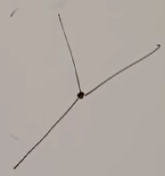
\includegraphics[width=0.8\textwidth]{split-particle1}
\end{figure}

\begin{align*}
\bra{k_1^\prime,k_2^\prime}&\int \Psi^\dagger(x)\Psi^\dagger(x)\Psi(x) dx\ket{k}\\
=&\bra{k_1^\prime,k_2^\prime}\int a^+(k_1^\prime) a^+(k_2^\prime) a^-(k) \underbrace{e^{ikx} e^{-i(k_1^\prime+k_2^\prime)x}}_\text{integrates to Dirac-$\delta$--(\ref{eq:conservation:energy})} dx\ket{k}
\end{align*}

So invariance under space translation yields conservation of momentum.

Another possible symmetry: $\Psi \rightarrow e^{i \lambda} \Psi$: no change to probabilities if number of $\Psi$s is same as number of $\Psi^\dagger$s. This os connected with conservation of charge.

\subsection{Fermions}

\subsubsection{Introduction to Fermions}

\begin{itemize}
	\item Can have any number of Bosons in same state (same place);
	\item They have a tendency to be in same state. E.g. particles decays and emits photon. If lots of other photons already on some state, decay will preferentially favour that state.
\end{itemize}

Fermions cannot be in same state (Pauli Exclusion Principle).

\begin{align*}
\Psi(x) =& \sum_k a^-(k) e^{ikx}\\
State:& \ket{001...01010...} \text{, ones and zeroes only!}\\
\Psi^\dagger(x) =& \sum_k a^+(k) e^{-ikx}
\end{align*}

Focus on one state, either full $(\ket{1})$ or empty $(\ket{0})$: those are only two possibilities. What are the algebraic rules for creation and annihilation operators?

\begin{align*}
c^+\ket{0} =& \ket{1} \text{ for Fermions used $c$ rather than $a$}\\
c^+\ket{1} =& 0 \text{, i.e. $\psi(x) \equiv 0$}\\
c^-\ket{1} =& \ket{0}\\
c^-\ket{0} =& 0\\
\end{align*}

We deduce:
\begin{align*}
c^+c^-\ket{0} =& 0\\
c^-c^+\ket{0} =& \ket{0}\\
(c^+c^-+c^-c^+)\ket{0} =& \ket{0}\\
c^+c^-\ket{1} =& \ket{1} \\
c^-c^+\ket{1} =&0 \\
(c^+c^-+c^-c^+)\ket{1} =& \ket{1}\\
\{c^+,c^-\} =& 1 \text{, where anticommutator is defined}\\
\{c^+,c^-\} \triangleq(c^+c^-+c^-c^+)& \text{. We can also show}\\
\{c^+,c^+\} =&0 \text{ and}\\
\{c^-,c^-\} =&0
\end{align*}

So Fermions have parallel mathematics: $[,] \leftrightarrow \{,\}$. Cannot put two particles into same state, as $c^+c^+=0$.

What about different momenta? We can show that:
\begin{align*}
\{c^+_k,c^-_{k^\prime} \} =& \delta_{k,k^\prime} \\
\{c^+_k,c^+_{k^\prime} \} =&0 \\
\{c^-_k,c^-_{k^\prime} \} =&0
\end{align*}

Can we have two Fermions at the same position? Let's try to create them at the origin.

\begin{align*}
\Psi^\dagger(0) \Psi^\dagger(0) \ket{0} =& \sum_{k,k^\prime} c^+_k c^+_{k^\prime} \ket{0}\\
=& 0
\end{align*}

So the answer is no: we can't have two Fermions at the same position. So we can't have an electron laser.

\subsubsection{Ground State}
We now compare the ground state of a system of Bosons with the ground state of a system of Fermions. In Figure \ref{fig:electons:confined:momentum} we have some particles confined in momentum space.

\begin{figure}[H]
	\caption{Particles confined in momentum space (3D)}\label{fig:electons:confined:momentum}
	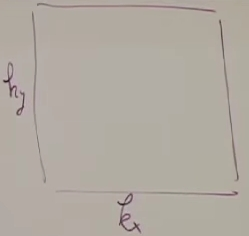
\includegraphics[width=0.8\textwidth]{electons-confined-momentum}
\end{figure}

Allowable values form a lattice.
\begin{itemize}
	\item We can put lots and lots of Bosons in the lowest energy (zero momentum), giving a Bose condensate. Complete uncertainty of position.
	\item Have to assign different momentum to electrons--Figure \ref{fig:adding:more:fermions}. Many Fermion configuration has much more energy that corresponding Boson configuration. 
\end{itemize}


\begin{figure}[H]
	\caption{Adding more Fermions}\label{fig:adding:more:fermions}
	\begin{subfigure}{0.32\textwidth}
		\caption{Two electrons, lowest possible energy}\label{fig:electons:lowest:energy}
		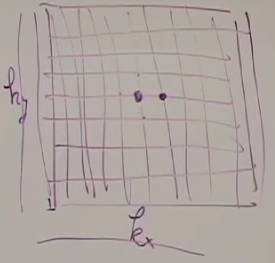
\includegraphics[width=0.9\textwidth]{electons-lowest-energy}
	\end{subfigure}
	\begin{subfigure}{0.32\textwidth}
		\caption{Filled lowest two energy levels.}
		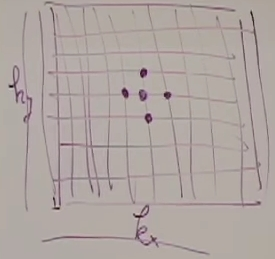
\includegraphics[width=0.9\textwidth]{5-electrons}
	\end{subfigure}
	\begin{subfigure}{0.32\textwidth}
		\caption{$E=\frac{k^2}{2m}$, so there are more positions in each energy level as energy increases.}
		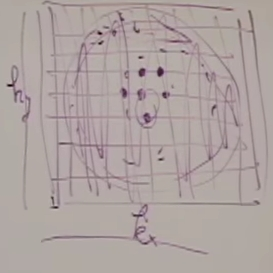
\includegraphics[width=0.9\textwidth]{more-fermions}
	\end{subfigure}
\end{figure}

\begin{defn}[Fermi Sphere]
	Electrons fill a sphere in momentum space, whose radius depends on number of electrons. This is called the Fermi Sphere.
\end{defn}

We can move Bosons and Fermions out of the ground state, as shown in Figures \ref{fig:bosons:move:ground:state} and \ref{fig:fermions:move:ground:state}.
\begin{figure}[H]
	\caption{Moving Bosons and Fermions from lowest state}
	\begin{subfigure}{0.5\textwidth}
		\caption{Bosons in Ground State}\label{fig:bosons:move:ground:state}
		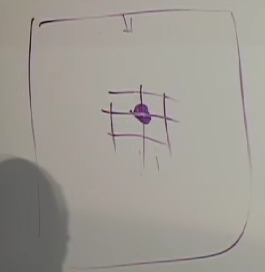
\includegraphics[width=0.9\textwidth]{bosons-ground-state}
	\end{subfigure}
	\begin{subfigure}{0.5\textwidth}
		\caption{Moving Fermions. Take from surface of Fermi Sphere to minimize energy required. Leaves hole behind.}\label{fig:fermions:move:ground:state}
		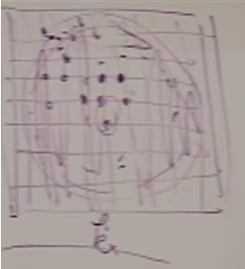
\includegraphics[width=0.9\textwidth]{moving-outside-fermi}
	\end{subfigure}
\end{figure}

In Figure \ref{fig:fermions:move:ground:state} a charged hole is left behind.
If an electron drops into hole, a photon is emitted.

Consider atom, al electrons in their ground state. Low energy electron is struck by photon, which takes electron to excited state.

\begin{defn}[Fermi Sea]
	Electrons in Fermi Sphere are said to be in Fermi Sea.
\end{defn}

Electrons that are deep in Fermi Sea can't be excited by low energy photons. Only shallow electrons are accessible.

\subsubsection{Dirac and antiparticles}

We consider the 1-dimensional case. Imagine a wave propagating to the tight with speed $c$.
\begin{align*}
\omega =& k\\
\frac{\partial \psi}{\partial t} =& - \frac{\partial \psi}{\partial x} \text{, would not make sense for Bosons.}\\
\psi =& e^{i(kx-\omega t)}
\end{align*}
What if $k$ negative? Then we have negative energy. But if we had arbitrarily negative energies, we could keep emitting photons all the way down.

Dirac said to fill all negative energy states: so lowest energy state has all negative energies filled. Now we can take an electron out, leaving hole. Now we have two positive energy objects, electron and positron.




\section{Dirac equation and Higgs particles}

\section{Angular momentum}

\section{Spin}

\section{Equations of motion of particles and fields}

\section{Field Lagrangians and path integrals}


\end{document}
